\documentclass[addpoints]{exam}
\usepackage[utf8]{inputenc}
\usepackage[portuguese]{babel}
\usepackage[LGRgreek]{mathastext}
\usepackage{graphicx,graphics}
\usepackage{hyperref}

\footer{}{\thepage}{}
 
\pointpoints{ponto}{pontos}
\bonuspointpoints{ponto extra}{pontos extra}
 
\totalformat{Pregunta \thequestion: \totalpoints pontos}
 
\chqword{Pregunta}
\chpgword{Página}
\chpword{Pontos}
\chbpword{Pontos extra}
\chsword{Pontos obtidos}
\chtword{Total}

\hqword{Questão}
\hpgword{Página}
\hpword{Pontos}
\hsword{Pontos obtidos}
\htword{Total}

 
\begin{document}
 
\begin{center}
Eletrônica Básica II – EE640 U - Lista SPICE final
\end{center}
 
\vspace{5mm}
 
\noindent\makebox[0.72\textwidth]{Nome: \enspace\hrulefill}
\hfill
\makebox[0.2\textwidth]{RA: \enspace\hrulefill}

\vspace{5mm}

\noindent\makebox[0.72\textwidth]{Nome: \enspace\hrulefill}
\hfill
\makebox[0.2\textwidth]{RA: \enspace\hrulefill}

\begin{center}
A lista deve ser entregue até dia \textbf{01-01-1968}
\end{center}

\vspace{2mm}

\begin{center}
\gradetable[h][questions]
\end{center}

\vspace{2mm}

\begin{framed} 

Deverá  ser entregue um relatório contendo a descrição completa do projeto, evidenciando TODOS os cálculos realizados e toadas as etapas de simulação. comentar sobre possíveis diferenças entre a simulação e os cálculos do projeto.

\end{framed}

\begin{center}

\vspace{2mm}

Use o seu RA como \textit{\textbf{abcdef}}, exemplo: para 123456, ab=12, ef=56 e assim port diante.

\vspace{2mm}

Utilize 0 como 10, 00 como 100. RA = 002220, ab=100, f=10
\end{center}

\vspace{2mm}

\begin{center}
\textbf{SIMULAÇÃO DE UM AMPLIFICADOR CMOS DE 2 ESTÁGIOS}
\end{center}

\vspace{5mm}

A Figura apresenta um amplificador CMOS de 2 estágios. Usando o software de simulação SPICE, faça a simulação do circuito observando os critérios abaixo. O modelo do transistor deve obrigatoriamente ser alterado. Use os seguintes parâmetros:

\vspace{2mm}

$\vert V_t \vert = 0,5$ V, $k'_p = k'_n = 10$ $\mu A/V^2$, $\lambda = 0,01$ $V^{-1}$, L = 1 $\mu m$, Cbd = 1 pF, Cgdo = 1 fF e Cgso = 1 fF.

\vspace{5mm}

\begin{questions}

\question No circuito da Figura identifique as seguintes partes: Fontes de Corrente, Carga ativa, Estágio de Entrada e Estágio de Saída

\question Calcule o valor de R1 para que a corrente de referência seja 10 $\mu A$ + (``ef'' $\times10^{-7}$)

\question Dimensione o primeiro estágio para um ganho de 100 + ``cd''.

\question Dimensione o segundo estágio para um ganho de 100 + ``de''.

\question Dimensione $M_3$ e $M_4$ para reduzir o \textit{offset}. Qual o menor valor de W/L que pode ser usado nesses transistores para garantir o funcionmanto do par diferencial?

\question Calcule $C_f$ para que a frequência $f_T$ seja 10 MHz + (``ce'' $\times10^5$). Localize os pólos e os zeros e estime a margem de fase.

\question Quais os valores máximos de tensão na saída? Por quê? Qual a máxima amplitude permitida na entrada? Compare os valores medidos com os teóricos.

\question Como você resolveria o problema do \textit{offset} encontrado?

\question Com o problema do \textit{offset} resolvido quais os novos valores máximos de tensão na entrada?

\question Construa um amplificador inversor com ganho ``bc''. Compare o ganho medido com o teórico.

\question Faça um \textit{datasheet} do seu amplificador que contenha as informações listadas a seguir. \textbf{Detalhar como cada um desses valores foi obtido :}

Ganho em malha aberta, tensão de\textit{ offset}, corrente de entrada, máxima variação de saída, máxima tensão de entrada, rejeição em modo comum, banda de passagem,\textit{ slew rate}, corrente consumida e potência consumida.



\begin{center}
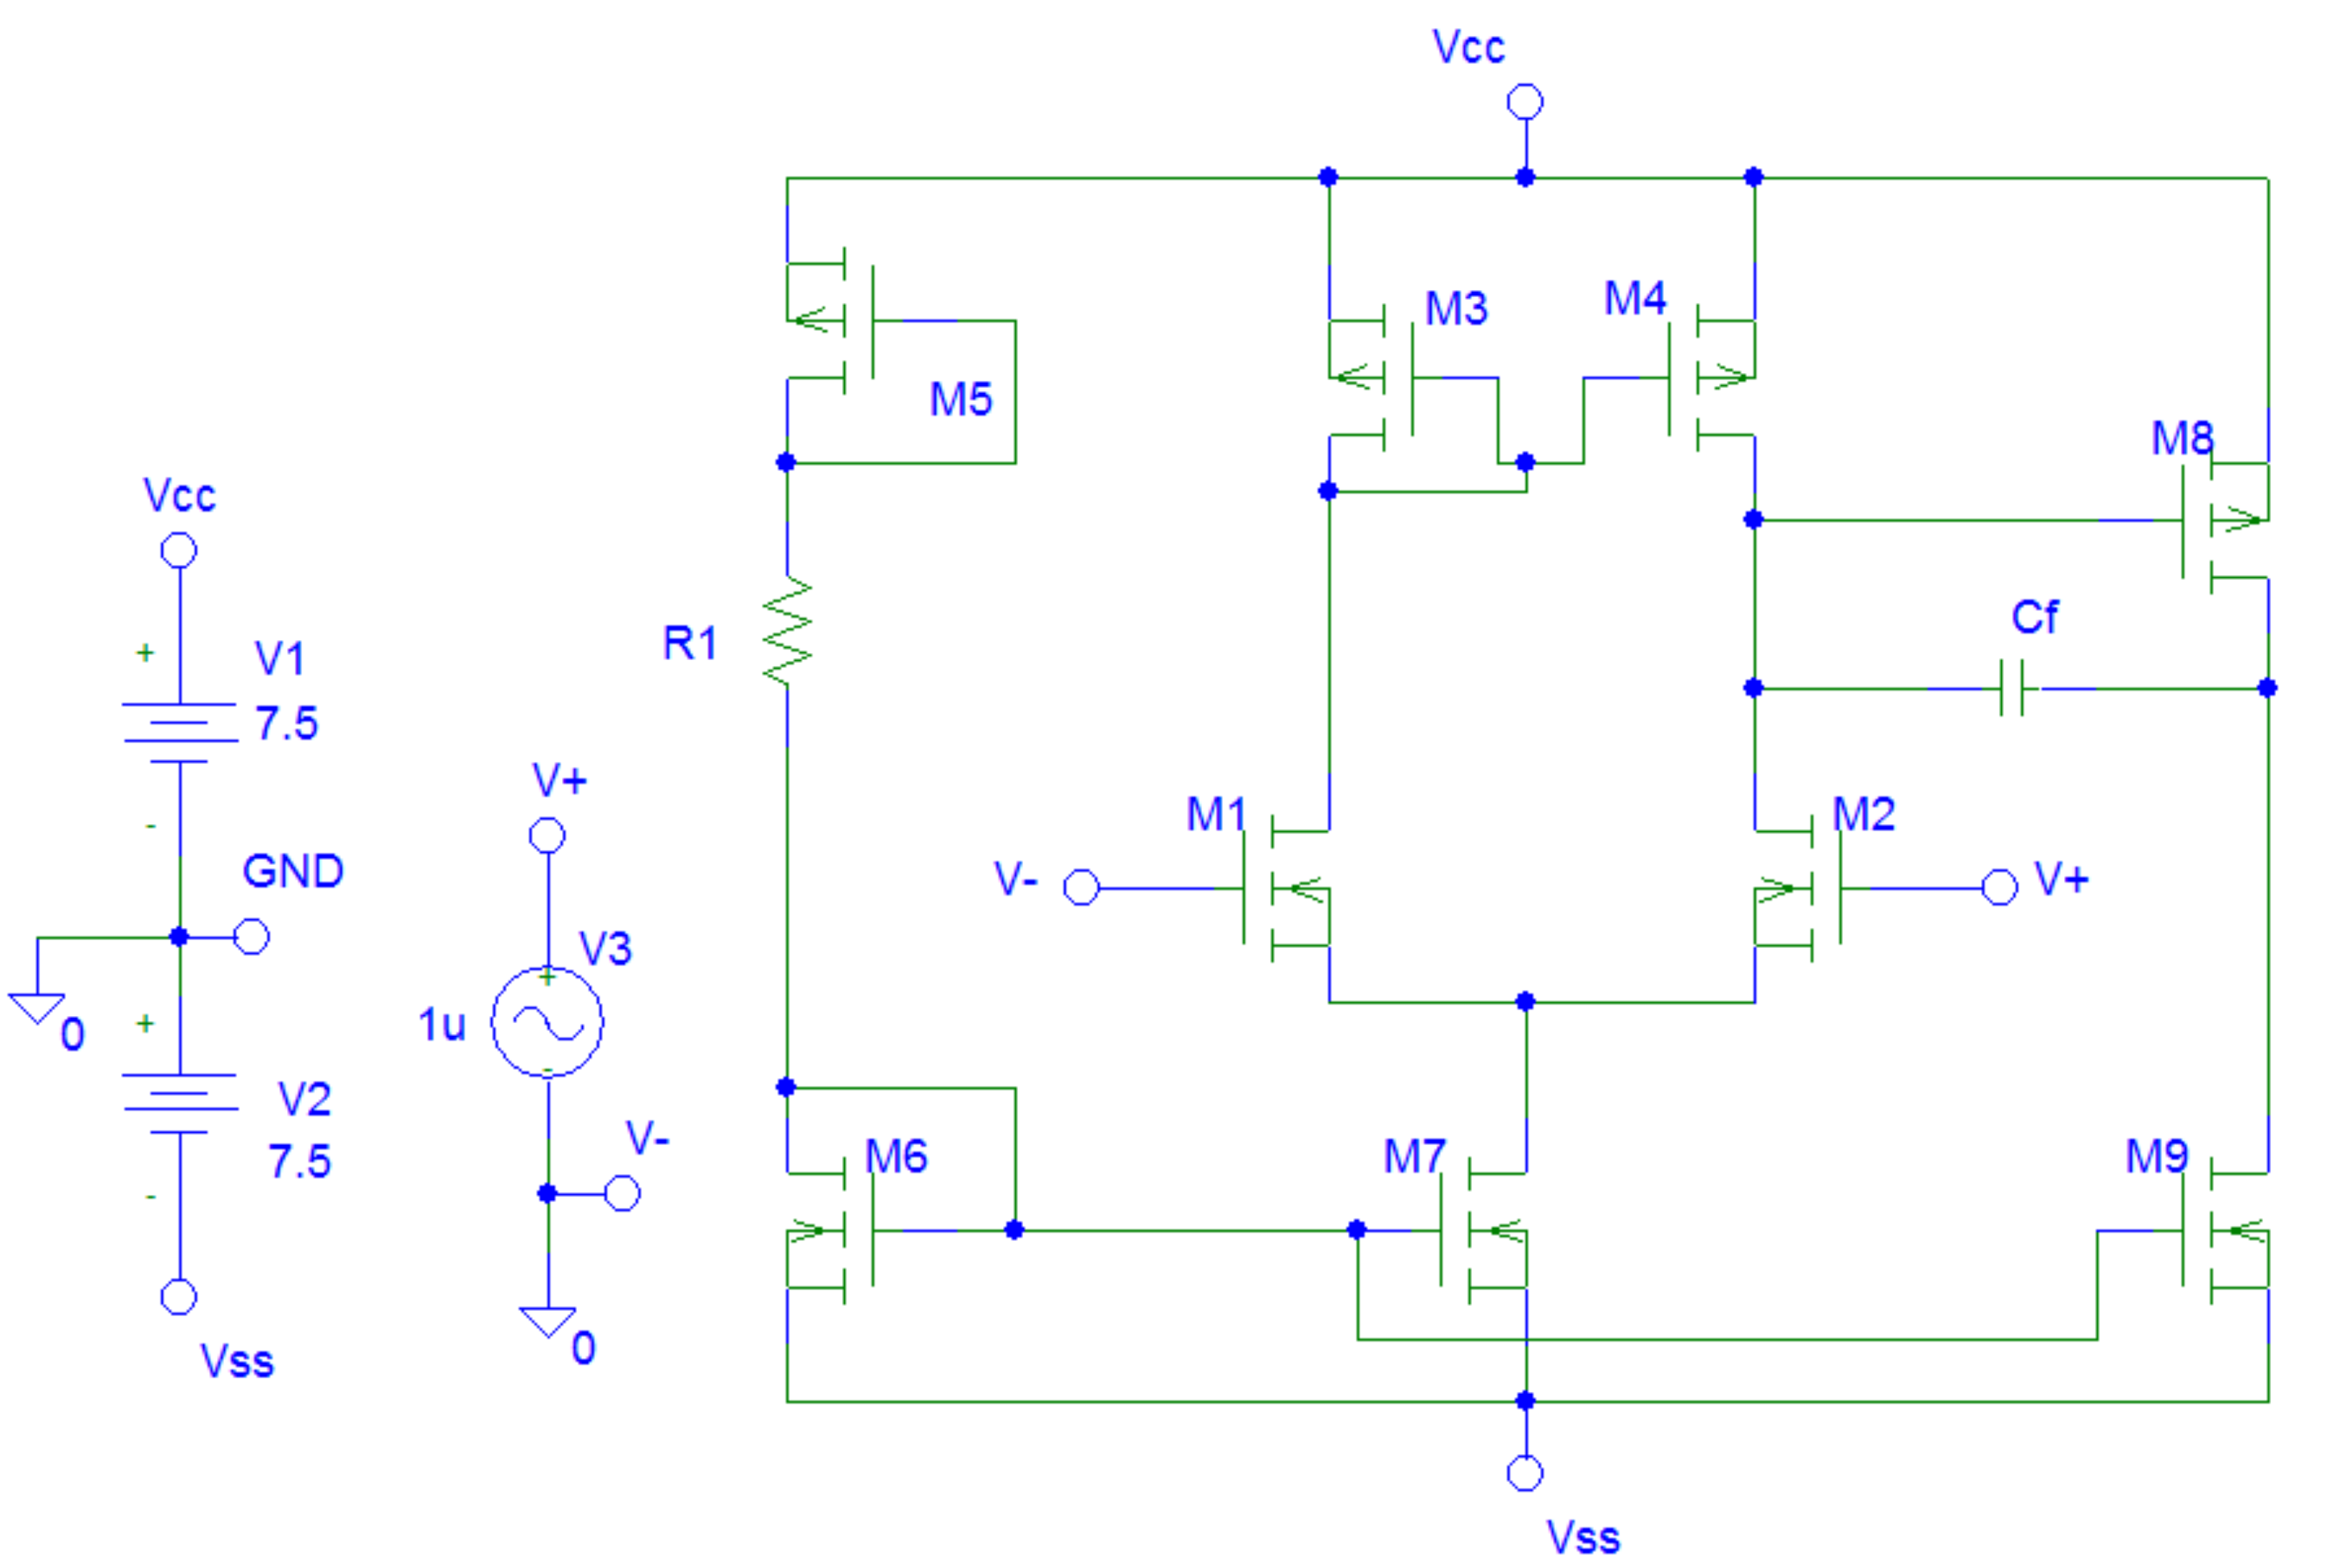
\includegraphics[width=0.9\textwidth]{imagens/1.png}
\end{center}



\vspace{5mm}

\textbf{REFERÊNCIAS}

\vspace{5mm}

MANERA, Leandro T. \textbf{Vídeos sobre SPICE}. \url{http://www.dsif.fee.unicamp.br/~manera/EE640/download.html}. Acesso em 08-01-2019.

UNIVERSITY OF PENNSYLVANIA. \textbf{Spice model parameters of mosfets}. \url{https://www.seas.upenn.edu/~jan/spice/spice.MOSparamlist.html}. Acesso em 08-01-2019.

\end{questions}

\end{document}
